\section*{Einleitung}
Ziel dieses Softwareprojektes ist es aus einem gegebenen Apollonianischen Netzwerk mit $n$ Knoten ein Gestapeltes Polytop zu erzeugen, das einerseits konvex ist und andererseits ganzzahlige Koordinaten besitzt. Dabei sollen die Koordinaten möglichst klein sein, das heißt maximal polynomielle Größe in der Eingabegröße $n$ besitzen. Es soll eine Software erstellt werden, in der man beliebige Apollonianische Netzwerke, wenn möglich grafisch, eingeben kann. Das Ergebnis - also das zugehörige Gestapelte Polytop - soll dann ausgegeben und angezeigt werden.\\
Um dies zu realisieren, werden beide Objekte in einer baumartigen Datenstruktur abgelegt. Da diese Datenstrukturen recht einfach sind, benutzen wir dazu keine fertigen Bibliotheken. Für die grafische Darstellung der Polytope benutzen wir die auf dreidimensionale und mathematische Visualisierung ausgerichtete Java Bibliothek JReality \cite{jreality}. Da die Software komplett in Java geschrieben wurde, bot sich die Einbindung dieser Bibliothek an.

\section*{Projektorganisation}
Da unsere Gruppe lediglich aus 5 Personen bestand, haben wir uns dazu entschieden eine sehr einfach gehaltene Projektstruktur anzulegen. Dazu haben wir das Projekt in 4 verschiedene Bereiche zerlegt, die größtenteils unabhängig voneinander bearbeitet werden konnten. Das Programm sollte nach dem EVA-Prinzip arbeiten, weshalb 3 der 4 Bereiche die Eingabe, Verarbeitung (d.h. Implementierung des Algorithmus) und Ausgabe sind. Diese konnten vollkommen unabhängig voneinander implementiert werden. Der 4. Bereich stellt die beiden Schnittstellen zwischen 2 Bereichen dar.\\
Um den Schnittstellen-Bereich sauber zu implementieren, haben wir uns wöchentlich im Institut getroffen. Bei diesen Treffen diskutierten wir meist mögliche Herangehensweisen und Probleme der 4 Bereiche. Die dabei entstandenen Lösungs-möglichkeiten wurden dem wöchentlichen Aufgabenkatalog hinzugefügt. Die Ergebnisse dieser Besprechungen und zukünftige Aufgaben hielten wir in einem Spline-Pad (\texttt{http://pad.spline.de}) fest. Damit hatten wir immer einen Überblick was noch getan werden musste und wie weit die anderen Bereiche sind. Mögliche Designfragen wurden hier ebenfalls diskutiert. Falls es Probleme gab, die nicht bis zum nächsten Treffen warten konnten, benutzten wir E-Mail-Verkehr um diese zu lösen.\\
Um den Quellcode organisieren zu können, benutzten wir das freie Tool GitHub (\texttt{https://github.com}). Dieses Tool ermöglicht es, parallel am selben Quelltext zu arbeiten ohne dass es zu Informationsverlust kommt. Über dieses Tool haben wir unser Projekt gehostet. Da die meisten Bereiche unabhängig voneinander waren, ist es meistens nicht nötig gewesen, unterschiedliche Branches zu verwenden. Auf dem Master-Branch lag daher immer eine kompilierbare Version des Projektes mit mehreren Main-Methoden.

\section*{Der Algorithmus und die mathematischen Grundlagen}
Wir betrachten im folgenden ein Apollonianisches Netzwerk und wollen verstehen was das ist. Dazu sei $G=(V,E)$ ein planarer Graph, den wir in den $\R^2$ zeichnen. Möchte man einen Knoten $v$ in den Graphen an Stelle $p\in\R^2$ einfügen, so werden alle Knoten mit $v$ mit einer Kante verbunden, solange diese dafür sorgen, dass $G$ planar bleibt. Startet man mit dem vollständigen planaren Graphen $K_3$ und fügt wie beschrieben nacheinander Punkte ein, so ist der entstandene Graph ein Apollonianisches Netzwerk.\\
Die Definition eines Gestapelten Polytops verhält sich ähnlich. Dabei gehen wir wieder von einem Dreieck aus, welches sich diesmal im $\R^3$ befindet. Bei einer Stapeloperation werden drei Punkte des Polytops genommen, die paarweise adjazent sind. Diese 3 Punkte werden alle mit einem neuen Punkt verbunden und bilden zusammen ein Tetraeder. Ein Polytop ist gestapelt, wenn es durch eine Folge solcher Stapeloperationen entstanden ist.\\
Wir haben den folgenden Satz aus \cite{stackedPoly1}:

\begin{thm}
Sei $G$ ein Apollonianisches Netzwerk mit $n$ Knoten. Dann kann $G$ als $3$-dimensionales konvexes gestapeltes Polytop mit ganzzahligen Koordinaten realisiert werden, das höchstens die Größe $2160n^4\times 2160n^4\times 162n^6$ besitzt.
\end{thm}

Da es äußerst kompliziert erschien, die im Beweis verwendeten Fachbegriffe in ein sinnvolles Deutsch zu übersetzen, verweisen wir an dieser Stelle auf unseren Anhang A. Henrique Hepp hat dort den zugrunde liegenden Algorithmus auf Englisch zusammengefasst. Dieser wurde auch so implementiert.

\section*{Die Umsetzung}
Wie bereits erwähnt haben wir die Software in mehrere Teile zerlegt, unter anderem die Eingabe, die Ausgabe und den Algorithmus. Aus dieser Zerlegung resultierte ein pipeline-artiger Informationsfluss, der wohldefinierte Schnittstellen benötigt. Wir betrachten zuerst diese wesentlichen Schnittstellen. Danach sollen die Bereiche Eingabe und Ausgabe genauer beleuchtet werden. 

\subsection*{Die Schnittstellen}
Wir haben zu klären, wie die beiden Objekte Apollonianisches Netzwerk und Gestapeltes Polytop in eine Java-Datenstruktur umgewandelt werden. Im Beweis wurde verlangt, dass man das Apollonianische Netzwerk als Baum darstellt, dessen Knoten die einzelnen Flächen darstellen. Ein innerer Knoten hat die drei Flächen als Kinder, die entstanden sind, nachdem eine Einfüge-Operation durchgeführt wurde. Wir verwenden diese baumartige Struktur, da somit gleich eine sinnvolle Eingabe für den Algorithmus gegeben ist. Dazu betrachte das folgende Inerface $Face$.

\begin{lstlisting}[language=Java, caption={Ausschnitt aus dem Face-Interface}]
public interface Face {
   public void merge();
   public void divide(PointDecimal p);
   public boolean isSmallestFace();
   public Face[] smallerFaces();
   public Face outerFace();
   public PointDecimal[] getPoints();
   public boolean hasPoint(PointDecimal p);
}
\end{lstlisting}

Die ersten beiden Methoden (merge,devide) sind nötig, um das Apollonianische Netzwerk zu manipulieren, d.h. Punkte zu löschen oder einzufügen. Die nächsten 3 Funktionen sind nötig um die Datenstruktur durchlaufen zu können (sowohl nach unten als auch nach oben im Baum). Für die grafische Eingabe ist es zudem notwendig, Punkte innerhalb des Netzwerkes zu bestimmen, da hier mit einer Point-and-Click-Methode gearbeitet werden soll. Dafür sind die letzten beiden Methoden notwendig. Das Interface besitzt noch weitere Methoden, die wir hier nicht alle aufführen wollen und größtenteils nur zur Hilfe im Algorithmus verwendet werden. Zusammen mit dem nächsten Interface kann man die Java-Dateien im Package $interface$ finden. Das Interface für die Gestapelten Polytope ist ähnlich aufgebaut und soll daher nicht genauer erläutert werden. Hier wird ebenfalls nur eine Auswahl der wichtigsten Methoden getroffen.

\begin{lstlisting}[language=Java, caption={Ausschnitt aus dem StackedPolytope-Interface}]
public interface StackedPolytope {
   public void merge();
   public void divide(PointInteger p);
   public boolean isBoundary();
   public StackedPolytope[] smallerPolytopes();
   public StackedPolytope baseTriangle();
   public PointInteger[] getPoints();
}
\end{lstlisting}

\subsection*{Die Eingabe}
Im Fokus stand an dieser Stelle, wie man den Benutzer Apollonianische Netzwerke eingeben lassen kann. Zum einen soll dies mit einer grafischen Oberfläche funktionieren. Dazu bekommt der Benutzer den vollständigen Graphen $K_3$ gezeigt und kann nun in diesem Dreieck nach Belieben weitere Punkte einfügen oder löschen. Aus dem dargestellten Netzwerk wird dann das Gestapelte Polytop berechnet. Zudem können bereits gezeichnete Netzwerke in Dateien gespeichert werden, die man dann erneut laden kann. Für das grafische Benutzerinterface benutzen wir die Java-Bibliothek Swing \cite{swing}. Im Package $input$ stehen dazu alle nötigen Klassen bereit.\\
Da mit dieser Methode jedoch nur sehr kleine Netzwerke möglich sind, mussten wir uns eine zweite Variante ausdenken, wie man vor allem größere Netzwerke als Eingabe nutzen kann. Der Benutzer kann mithilfe einiger Argumente hinter dem Programmaufruf mehrere Polytope unterschiedlicher Größe berechnen lassen. Im folgenden Listing haben wir eine Zusammenstellung dieser Befehle.

\begin{lstlisting}[caption={Kommandozeilen-Befehle}]
// Keine Argumente - startet die GUI
java -jar The_Polytopelizer.jar

// ? - zeigt das Hilfemenue
java -jar The_Polytopelizer.jar ?

// Siehe Hilfemenue fuer Beschreibung dieser 3 Befehle
java -jar The_Polytopelizer.jar random <n> <m>
java -jar The_Polytopelizer.jar rate <n> <m>
java -jar The_Polytopelizer.jar <input.aN> <Output.pol>

\end{lstlisting}

Das Package $main$ enthält die Klassen, die für diese Aufgabenzuweisung nötig sind. Abbildung \ref{apollNet} zeigt die Eingabe-Umgebung mit einem Apollonianischen Netzwerk, bestehend aus 8 Knoten.

\begin{figure}[htbp]
	\centering
	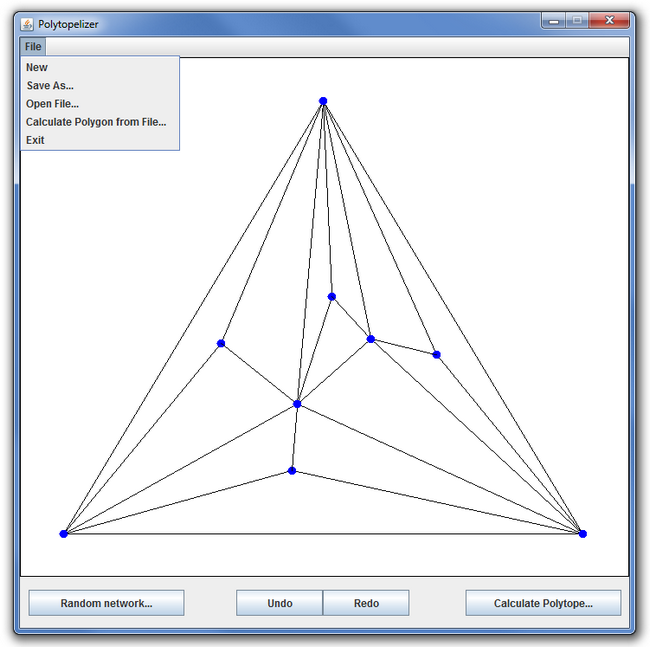
\includegraphics[scale=0.5]{figures/input.png}
	\caption{Ein Apollonianisches Netzwerk mit 8 Knoten.}
	\label{apollNet}
\end{figure}

\textbf{Probleme} Während der Entwicklung der Eingabe kam es des öfteren zu Problemen mit der Face-Schnittstelle. Diese wurde anfangs nicht ganz korrekt implementiert. Erst beim Testen der GUI konnten Fehler in der Implementierung dieser Schnittstelle festgestellt werden. Diese zu finden, war oft sehr mühselig. Zudem war lange Zeit unklar, ob das grafisch dargestellte Netzwerk skalierbar sein soll oder nicht. Damit hätte der Benutzer im Netzwerk rein und rauszoomen können und wäre in der Lage gewesen mehr Punkte genauer zu setzen. Diese Idee wurde jedoch irgendwann verworfen, weil auch ohne zoomen hinreichend viele Punkte genau gesetzt werden können und außerdem durch das CLI andere Möglichkeiten gegeben waren, Polytope mit sehr vielen Ecken zu berechnen. Zudem war unklar, ob man mit dem verwendeten Datentyp BigDecimal für die Darstellung von Gleitkommazahlen das Setzen von Punkten in stark hereingezoomten Netzwerken ohne größeren Aufwand realisieren kann.

\subsection*{Die Verarbeitung}
Auf den Aspekt der Verarbeitung gehen wir nur sehr kurz ein, da der Algorithmus bereits behandelt wurde. Der Algorithmus an sich befindet sich im Projekt in einer einzigen Klasse, die austauschbar ist. In den Artikeln \cite{stackedPoly1} und \cite{stackedPoly2} werden zwei unterschiedliche Algorithmen beschrieben, die unterschiedliche Schranken für die Größe des Polytops aufweisen. Wir haben uns für den 1. Algorithmus entschieden, da dieser einfacher zu verstehen und somit einfacher zu implementieren war. Zudem sind die Schranken besser als beim 2. Algorithmus. Wir planten auch den zweiten Algorithmus zu implementieren, jedoch fehlte uns dafür die Zeit. Interessant wäre gewesen, ob dieser wirklich schlechter als der erste ist. Die Grenzen, die beim 1. Algorithmus laut Artikel berechnet wurden, konnten von uns nachgewiesen werden. In beiden Fällen sind die Schranken jedoch groß genug um selbst für kleines $n$ aus dem Darstellungsbereich von Integer oder Double herauszukommen. Aus diesem Grund nutzten wir die Datentypen $BigInteger$ und $BigDecimal$, die von Java zur Verfügung gestellt werden. Mit ihnen ist es möglich beliebig große Zahlen mit beliebig großer (jedoch endlicher) Genauigkeit abzuspeichern.

\subsection*{Die Ausgabe}
Im Bereich der Ausgabe mussten wir uns darum kümmern, wie man ein gestapeltes Polytop am besten darstellt. Die Java-Bibliothek jReality bot dazu eine umfassende Möglichkeit an, das Polytop grafisch darzustellen. Es ist damit möglich, das Objekt zu drehen oder zu zoomen. Zudem können die Frames von Jreality auch in die Swing-Oberflächen von Java eingebettet werden. Außerdem besitzt unsere Software die Möglichkeit sämtliche Punkte als Liste anzuzeigen oder abzuspeichern. Im Package $output$ ist die Klasse $Transformation.java$ dafür zuständig ein Gestapeltes Polytop zu iterieren um dessen Punkte und Kanten dann für jReality zur Verfügung zu stellen. Die anderen Klassen sind dann dafür da, das Polytop anzuzeigen und die Operationen zur Verfügung zu stellen (als Bild oder als Punktliste speichern). In Abbildung \ref{polytop} sehen wir die Ausgabe-Oberfläche mit dem zugehörigen Gestapelten Polytop aus Abbildung \ref{apollNet}.\\

\begin{figure}[htbp]
	\centering
	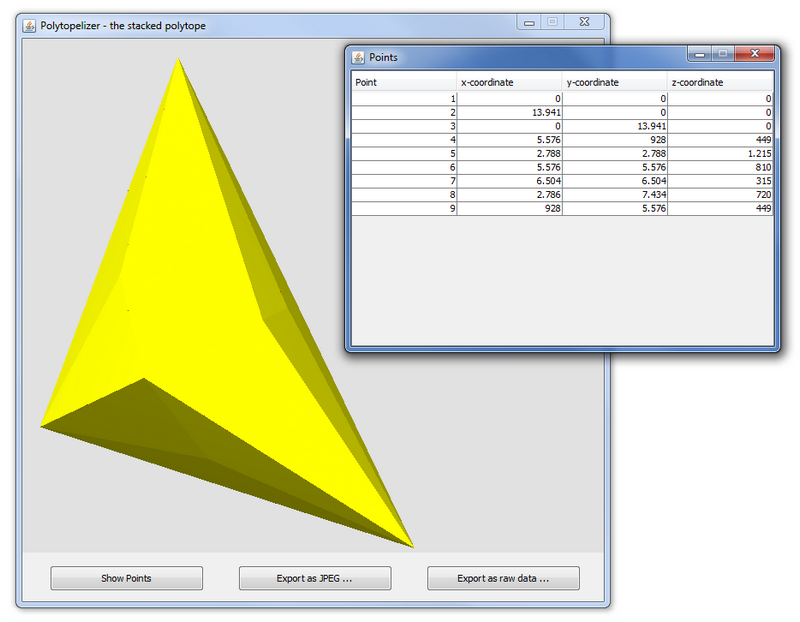
\includegraphics[scale=0.5]{figures/output.png}
	\caption{Darstellung des Polytops (links) und die zugehörige Punktliste (rechts)}
	\label{polytop}
\end{figure}

\textbf{Probleme} Ein großes Problem stellte die Verwendung von jReality dar, da die Bibliothek nicht genügend dokumentiert wurde. Durch viele Grafiken war uns zwar klar, dass sie alle Funktionen bereitstellen würde, die wir benötigen, jedoch war es nur durch eine intensive Suche über Suchmaschinen oder im Quelltext selbst möglich herauszufinden, wie man jReality einbinden kann. Im Endeffekt stellte sich dann heraus, dass die Einbindung recht einfach ist. Da uns jedoch andere Kommiliton(inn)en empfohlen haben, diese zu nutzen, haben wir uns mit dessen Funktionsweise genauer beschäftigt. Zudem waren andere Bibliotheken noch schlechter dokumentiert.\\
Ein anderes Problem war die Größe der Polytops. Da diese vor allem für große $n$ sehr groß werden, ist es eigentlich unmöglich, diese noch sinnvoll anzuzeigen. Eine Aushilfe soll dabei die Liste der Punkte schaffen. Mit diesen Punkten kann man sich wenigstens einen Überblick darüber verschaffen, in welchen Dimensionen sich das Polytop befindet. Eine Möglichkeit dieses Problem zu lösen, wäre es gewesen, eine Koordinatenachse zu stauchen. Wir haben uns jedoch dagegen entschieden, weil dies das eigentliche Resultat des Algorithmus verzerren würde. Zudem gibt es Programme (z.B. GNU-Plot \cite{gnuplot}), die die als Liste gespeicherten Punkte des Gestapelten Polytops anzeigen können - jedoch mit Stauchung einer Achse.

\section*{Fazit}
Es wurde eine Software erstellt, die aus Apollonianischen Netzwerken Gestapelte Polytope berechnet, die konvex sind und zudem kleine ganzzahlige Koordinaten besitzen. Zu diesem Zweck wurden Java Swing und jReality für eine GUI kombiniert. Den Algorithmus und die dazugehörigen Datenstrukturen implementierten wir selbst.\\

\textbf{Erreichte Ziele} Das Visualisieren von Apollonianischen Netzwerken und Gestapelten Polytopen konnten wir erfolgreich umsetzen. Zudem funktioniert der Algorithmus korrekt. Probleme haben wir jedoch bei sehr großen Koordinaten, bei denen das Gestapelte Polytop nicht mehr sinnvoll angezeigt werden kann. Zu diesem Zweck haben wir Möglichkeiten für eine Ein- und Ausgabe implementiert, die keine GUI benötigt.\\

\textbf{Allgemeine Probleme} Die Bereich-spezifischen Probleme haben wir bereits aufgeführt. Zudem kamen jedoch Probleme in der allgemeinen Organisation. Für fast alle von uns war dieses Softwareprojekt das erste. Der eigene Quelltext wurde zu wenig kommentiert, sodass häufig viele Stellen persönlich erklärt werden mussten. Außerdem kam es an einigen wenigen Stellen dazu, dass Quellcode überflüssig war. Vermutlich lässt sich der Quelltext daher in einigen Bereichen noch optimieren.\\ Bedauerlicherweise haben wir uns nicht an die aufgeschriebenen Meilensteine gehalten, sondern die einzelnen zu implementierenden Punkte immer weiter hinausgezögert. Somit kam es am Ende des Semesters zu mehr Arbeit. Dieses Phänomen ist aus der Softwaretechnik bekannt und tritt oft bei Anfängern auf.\\
Ein weiteres großes Problem war das Verständnis der mathematischen Grundlagen des Algorithmus. Hier kam es immer wieder zu Missverständnissen, die eine falsche Implementierung zur Folge hatten.\\

\textbf{Sonstiges} Viele allgemeine Erfahrungen konnten während des Projekts gemacht werden. So ist es zum Beispiel unverzichtbar, sich wöchentlich mit der Gruppe zu treffen. Hier kann man über mögliche Lösungsansätze diskutieren und sich gegenseitig auf den neusten Stand bringen. Die Projektarbeit wird dadurch motiviert, dass man Erfahrungen austauschen kann. Die Verwendung mit GitHub funktionierte zudem sehr gut, da man hier eine gute Versionsverwaltung hatte und gemachte Fehler einfach rückgängig machen kann. Zudem ist während der Verwendung des Algorithmus aufgefallen, wie wichtig Tests doch sind. Vermutlich wäre es sogar besser, erst bestimmte Tests zu schreiben und dann die Klassen zu implementieren.\\

\textbf{Offengebliebenes} Einige Aspekte müssen jedoch offen bleiben, die für eine Verbesserung der Software in Frage kommen würden. Wie ist es z.B. möglich, die GUI zu verändern, sodass diese noch benutzerfreundlicher wird? Wie schlägt sich der implementierte Algorithmus mit anderen? Bestimmt ist es möglich noch mehr aus der Bibliothek jReality herauszuholen, sodass die Polytope noch besser angezeigt werden können.

\chapter*{Anhang A - Der Algorithmus}

The algorithm can be divided in:

\begin{enumerate}
\item Receive the entry.
\item Heavy caterpillar decomposition.
\item Balance the tree.
\item Calculate the shifts.
\item Calculate new coordinates.
\item Lift the graph to a polytope. 
\item Round the graph to grid points.
\end{enumerate}
 

\section*{The Entry of the algorithm}

Given a $3$-connected planar graph and a tree representation of this graph, as shown below.

\begin{center}
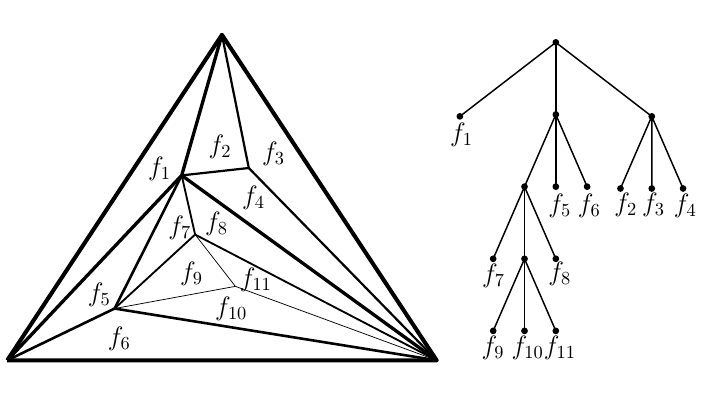
\includegraphics[scale=0.7]{./figures/graph_tree.png} 
\end{center}

\section*{Heavy caterpillar decomposition}
The tree representation is decomposed in \textit{heavy paths}. The resulting sub-trees are called \textit{caterpillars}. If a node lies on a heavy path it is called a \textit{spine node}, otherwise is a \textit{tree node}. The spine nodes are labelled by $s_1$ (root), $s_2$, ..., $s_i$,...,$s_\bot$. The children of $s_i$ are $s_{i+1}$, $t_{i+1}$ and $t'_{i+1}$. We store a pointer link in $t$ to another caterpillar - called $(t)$.

\begin{center}
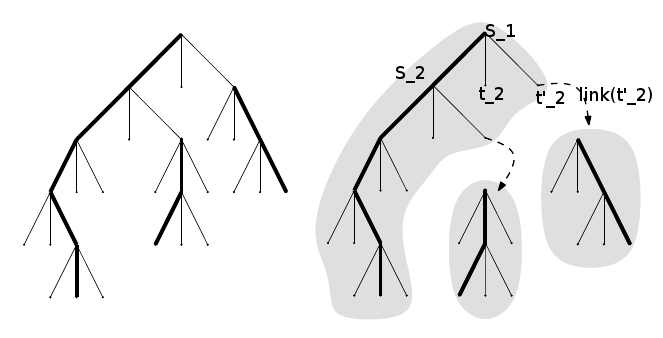
\includegraphics[scale=0.7]{./figures/caterpillarEdit.png} 
\end{center}

\section*{Balance the tree}

The pseudocode below shows the balancing of the tree.

\begin{algorithmic}
\Function{BALANCE}{C} 
\State \textbf{Input:} A caterpillar $C$ from the heavy caterpillar decomposition of $\tau(G)$. All weights are equal 1.
\State \textbf{Output:} Weights for the nodes of $\tau(G)$.

\If {isSmallestFace}
	\State return;
\Else
	\State BALANCE(($s_i$))
	\State BALANCE(link($t_i$))
	\State BALANCE(link($t'_i$))

	\If {$w(t_i)>w(t'_i)$}
        \State relabel $t_i \leftrightarrow t'_i$
	\EndIf

	\State $w(t_i)=w(t'_i)$
	
	\State $w(s_{i-1})$ = $w(s_i) + 2w(t_i)$ 
\EndIf
\EndFunction
\end{algorithmic}
A balanced tree has the following properties:

$$w(s_{i-1})= w(s_i) + w(t_i) + w(t'_i)$$

$$w(s_i)\geq w(t_i),w(t'_i) $$

$$w(t_i)= w(t'_i) $$

An example of a balanced tree is shown in the following graphic: 

\begin{center}
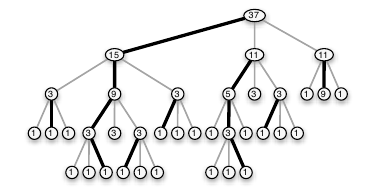
\includegraphics[scale=1]{./figures/balancedTree.png} 
\end{center}

\subsection*{Calculate the shifts} 

After stacking a vertex $v_i$ on a face $f_D$ , we get the new height:

$$z= \zeta_i + z_D $$

Where $z_D$ is the height of the point in the face $D$ and the shift $\zeta_i$ is:

$$\zeta_i = A_i\cdot B_i$$

Where  $ A_i$ and $B_i$ are the two possible weights of the three new faces formed by the vertex $v_i$. Remember $w(t_i)= w(t'_i) $.

But before we calculate the new heights ($z_i$) we round the coordinates in the embedding, and then the heights, too.

\subsection*{Calculate new coordinates}

The flat graph needs to have barycentric coordinates. In our case, the areas from the triangle has to be the values of the balanced tree. To calculate the new coordinates we use the formula: $P = t_1*A + t_2*B + t_3*C$, where $t_1$,$t_2$,$t_3$ are proportional to the areas in opposition to the points $A$,$B$,$C$.

\subsection*{Round the graph to grid points}

We have to round the coordinates on the embedding so that they are multiples of $1/\text{pert}$, where:

$$\text{pert}=240R^{\frac{3}{2}}$$

$R$ is the weight of the root from the balanced tree.

Now we lift, rounding, the points so that the heights $z= \zeta_i + z_D $ are multiples of $1/\text{pert}_z$, where: 

$$\text{pert}_z=3R$$ 

After these points are rounded they are still real numbers, not integers. To make them integer we multiply them with pert.

To round the coordinate we calculate:

$$\lfloor x\cdot\text{pert}\rfloor \div \text{pert}$$

To gain the final value in integer:

$$\lfloor x\cdot\text{pert}\rfloor \div \text{pert} \cdot\text{pert} = \lfloor x\cdot\text{pert}\rfloor$$

\begin{thebibliography}{999}
\bibitem {stackedPoly2} Erik D. Demaine und André Schulz, Embedding stacked polytopes on a polynomial-size grid, in Proceedings of the 22nd Annual ACM-SIAM Symposium on Discrete Algorithms (SODA 2011), San Francisco, California, USA, January 22–25, 2011, S. 1177–1187.
\bibitem {stackedPoly1} Erik D. Demaine und André Schulz, Embedding stacked polytopes on a polynomial-size grid, http://arxiv.org/abs/1403.7980, April 2014.
\bibitem {gnuplot} http://www.gnuplot.info/ Abgerufen am 1. Juni 2014.
\bibitem {jreality} http://www3.math.tu-berlin.de/jreality/ Abgerufen am 21. April 2014.
\bibitem {swing} http://docs.oracle.com/javase/6/docs/technotes/guides/swing/6.0/index.html Abgerufen am 24. April 2014.
\end{thebibliography}